\begin{tikzpicture}[
    box/.style={
        draw,
        rectangle,
        minimum width=4cm,
        minimum height=3cm,
        align=center,
        fill=gray!10,
        font=\small,
    },
    arrow/.style={
        ->,
        line width=0.5mm,
        >=latex
    }
]

% First two boxes
\node[box] (data) {Source dataset and\\input parameters\\ \\
    \begin{tikzpicture}[scale=0.5]
        % Main document
        \draw[fill=white] (0.1,0.1) -- (1.1,0.1) -- (1.1,1.4) -- (1.3,1.4) -- (1.3,0) -- (0.1,0) -- cycle;
        \draw[fill=darkgray!90] (0,0) rectangle (1.2,1.5);
        % Document lines
        \draw[black!30] (0.3,1.1) -- (0.9,1.1);
        \draw[black!30] (0.3,0.8) -- (0.9,0.8);
        \draw[black!30] (0.3,0.5) -- (0.9,0.5);
        % Second document        
        \draw[fill=white] (-0.3,-0.5) -- (0.7,-0.5) -- (0.7,0.8) -- (0.9,0.8) -- (0.9,-0.7) -- (-0.3,-0.7) -- cycle;
        \draw[fill=darkgray!90] (-0.4,-0.6) rectangle (0.8,0.9);
        % Document lines
        \draw[black!30] (-0.1,0.5) -- (0.5,0.5);
        \draw[black!30] (-0.1,0.2) -- (0.5,0.2);
        \draw[black!30] (-0.1,-0.1) -- (0.5,-0.1);

        \node[align=left, minimum width=3cm, minimum height=1cm, font=\tiny] at (4.5,0.5) {\textbf{Documents:} Accounting doc\\ \textbf{Inputs:} LLM, chunk size, ... \\ \textbf{Questions:} How are byproduct\\sales evaluated under Topic 606?\\...};
    \end{tikzpicture}
};

\node[box, right=0.6cm of data] (opt) {Run multi-objective\\optimization\\ \\
    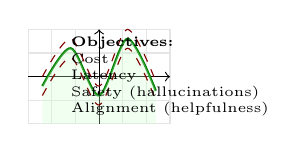
\begin{tikzpicture}[scale=0.6]
        % Background grid
        \draw[gray!20] (-1.5,-1) grid[step=0.5] (1.5,1);
        % Axis
        \draw[->] (-1.5,0) -- (1.5,0);
        \draw[->] (0,-1) -- (0,1);
        % Main optimization curve
        \draw[green!50!black, thick] plot [smooth] coordinates {(-1.2,-0.2) (-0.6,0.6) (0,-0.4) (0.6,0.8) (1.2,-0.3)};
        \fill[green!20, opacity=0.3] plot [smooth] coordinates {(-1.2,-0.2) (-0.6,0.6) (0,-0.4) (0.6,0.8) (1.2,-0.3)} -- (1.2,-1) -- (-1.2,-1) -- cycle;
        % Confidence intervals
        \draw[red!50!black, dashed] plot [smooth] coordinates {(-1.2,0) (-0.6,0.8) (0,-0.2) (0.6,1) (1.2,-0.1)};
        \draw[red!50!black, dashed] plot [smooth] coordinates {(-1.2,-0.4) (-0.6,0.4) (0,-0.6) (0.6,0.6) (1.2,-0.5)};

        \node[align=left, minimum width=2cm, minimum height=1cm, font=\tiny] at (1.5,0) {\textbf{Objectives:}\\Cost\\Latency\\Safety (hallucinations)\\Alignment (helpfulness)};
    \end{tikzpicture}
};

\node[box, right=0.6cm of opt] (pareto) {Select optimal configuration\\from pareto frontier\\ \\
    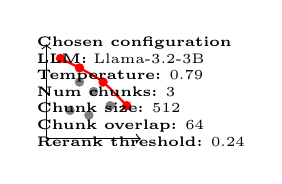
\begin{tikzpicture}[scale=0.6]
        \draw[->] (-1,-1) -- (1,-1);
        \draw[->] (-1,-1) -- (-1,1);
        \foreach \x/\y in {-0.5/-0.4, -0.1/-0.5, 0/0, -0.3/0.2, 0.35/-0.3}
            \fill[gray] (\x,\y) circle (0.1);
        \draw[red, thick] plot [smooth] coordinates {(-0.7,0.7) (-0.3,0.5) (0.2,0.2) (0.7,-0.3)};
        \foreach \x/\y in {-0.7/0.7, -0.3/0.5, 0.2/0.2, 0.7/-0.3}
            \fill[red] (\x,\y) circle (0.1);

        \node[align=left, minimum width=1.5cm, minimum height=1cm, font=\tiny] at (1,0) {\textbf{Chosen configuration}\\ \textbf{LLM:} Llama-3.2-3B\\ \textbf{Temperature:} 0.79 \\ \textbf{Num chunks:} 3\\ \textbf{Chunk size:} 512\\ \textbf{Chunk overlap:} 64 \\ \textbf{Rerank threshold:} 0.24};

    \end{tikzpicture}
};

% Arrows
\draw[arrow] (data) -- (opt);
\draw[arrow] (opt) -- (pareto);

\end{tikzpicture}